\documentclass{hipatia}



\subtitle{Memória}

\author{José Fernandes Silva Andrade}

\title{\fontsize{30}{30}\selectfont A Matemática na Minha Vida}

%Professor Aposentado do Departamento de Matemática da UFBA
\newcommand{\superau}{\textsuperscript{\underline{a}}~}
\newcommand{\superou}{\textsuperscript{\underline{o}}~}
\hyphenation{CAPES}
\hyphenation{gradua-ção}
\hyphenation{coorde-na-ção}
\hyphenation{coorde-na-dor}
\hyphenation{ex-pe-riên-cia}
\begin{document}
\setcounter{page}{\memoriapage}
\maketitle


\section{Apresentação}



Neste artigo, quero apresentar um pouco da minha trajetória
na área de Matemática. 
Como professor da UFBA, desempenhei
atividades de ensino, pesquisa, extensão e administração,
cada uma delas mais intensa em períodos diferentes, por
razões que incluem a própria evolução histórica do Instituto
de Matemática, atual Instituto de Matemática e Estatística.
Estas ponderações justificam dividir este artigo em períodos
cronológicos.



\section{Formação acadêmica}



\begin{center}\emph{1952--1970}\end{center}



Nasci em 23 de abril de 1952, em Salvador e, desde minha
infância, sempre gostei e tive muita facilidade para
Matemática. 
Fiz o curso secundário na escola pública: o 
ginásio foi cursado no Colégio Estadual João Florêncio Gomes,
de 1964 a 1967, e o científico no Colégio Central da Bahia,
de 1968 a 1970. Além do curso regular, estudei também
francês e inglês na Casa da França e no ACBEU,
respectivamente. 

Um ano antes de entrar na Universidade, sem conhecer direito
as perspectivas que teria ao fazer o Curso de Matemática,
através de meu pai, tive uma conversa excelente com a Profa.
Martha Dantas, professora de Matemática da Faculdade de
Educação, que além de me incentivar a fazer o Bacharelado em
Matemática, me falou da possibilidade de fazer cursos de
pós-graduação, mestrado e doutorado, e das perspectivas que
eu teria ao estudar em centros mais avançados. 

\begin{figure}[htb!]
\begin{center}
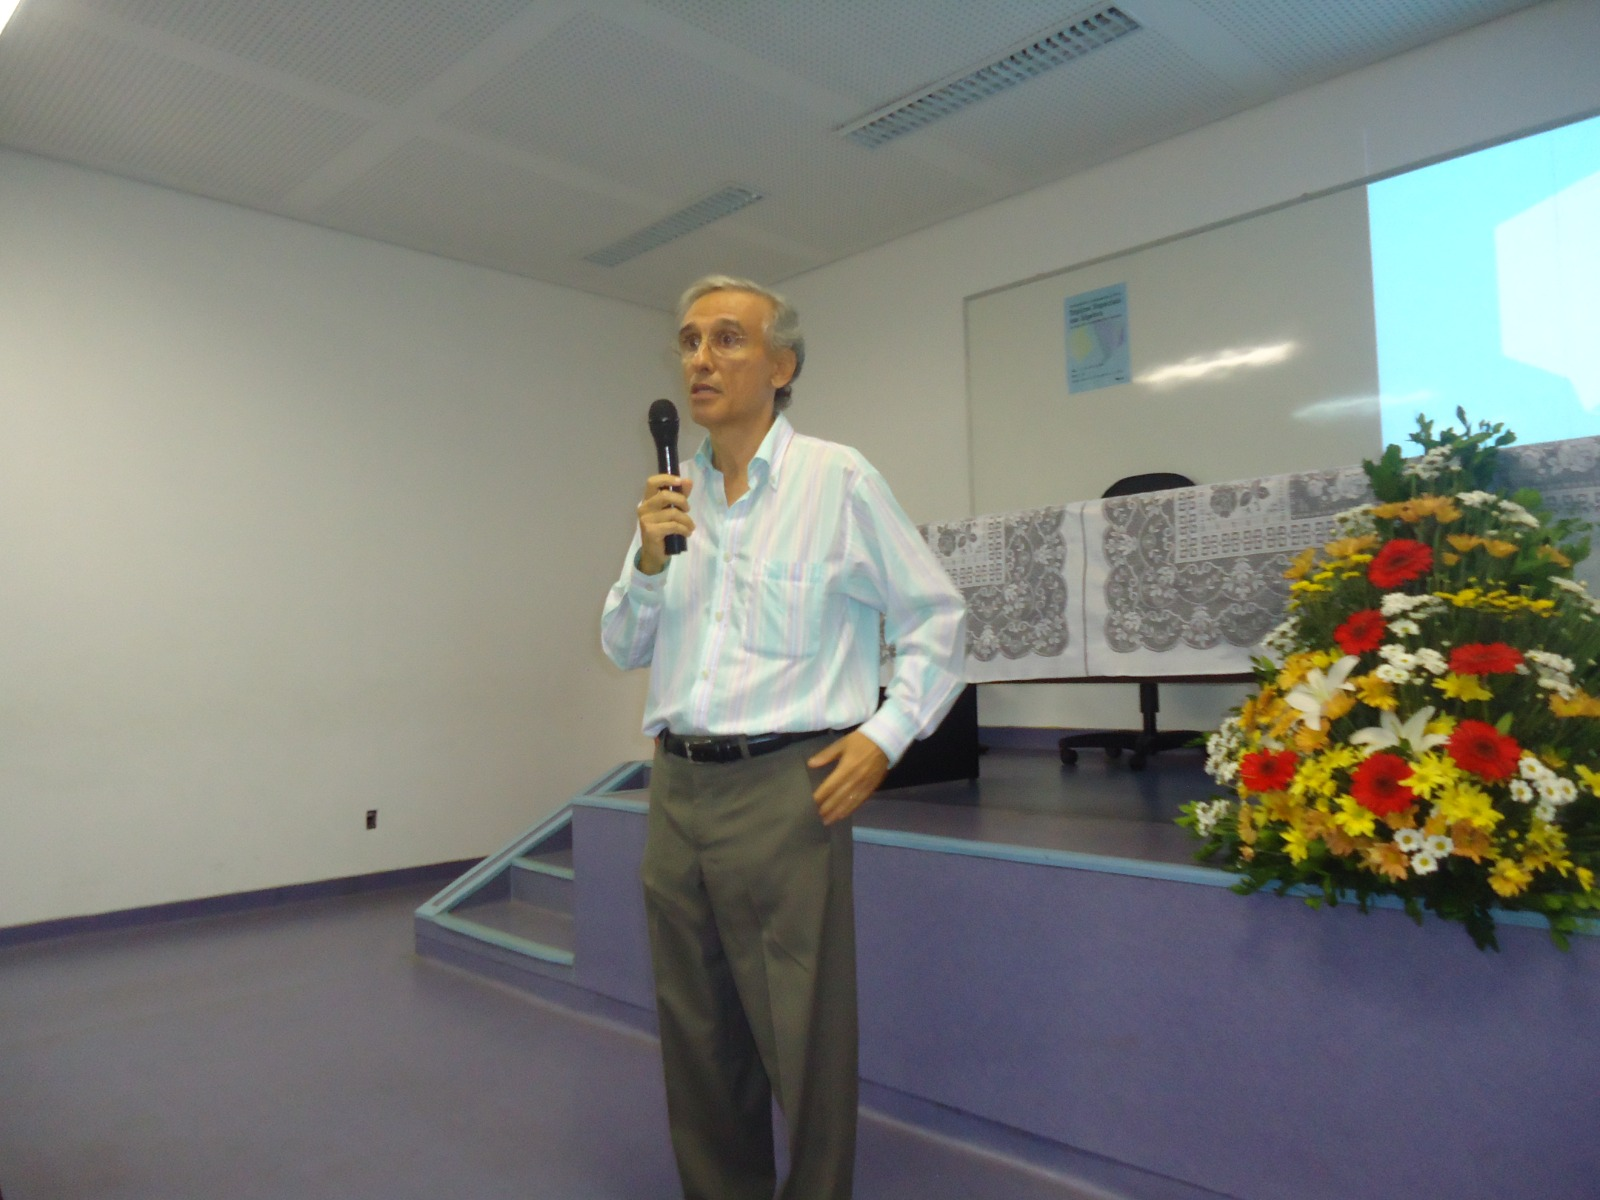
\includegraphics[width=8cm]{ZeFernandes.jpeg}
\end{center}
\caption{Prof. José Fernandes}   
\end{figure}

\begin{center}\emph{1971--1974 (UFBA)}\end{center}

Ingressei na Universidade Federal da Bahia, no princípio de
1971. Sabia que não seria um curso terminal, e que teria de
me preparar bem para as etapas seguintes que me aguardavam.
Logo no segundo semestre de 1971, fui aluno da Profa. Ana
Maria Costa, que me falou da possibilidade de obter uma
bolsa de iniciação científica do CNPq, e me apresentou ao
Prof. Omar Catunda. 
%%% reescrever o trecho abaixo? %/rev Henrique 
Fiz o pedido e, em abril de 1972, obtive a
resposta positiva da bolsa, sob a orientação do Prof.
Catunda, e deixei de ensinar no Colégio dos Servidores
Públicos, atividade que havia iniciado um ano antes, pouco
depois de ingressar na UFBA. 
Era mais do eu esperava para
aquela época, desenvolvendo outras atividades no Instituto
de Matemática, além do curso regular. No segundo semestre de
1972, como parte de minhas atividades na iniciação
científica, tive a oportunidade de dar aulas de exercícios
de Cálculo I, sob a orientação da Profa. Nina Rosa Braga,
que estava concluindo seu mestrado na UFBA.
%%sugestão%/revH e Elais
%\textcolor{red}
%{
%Fiz o pedido da bolsa e, em abril de 1972, obtive a resposta positiva, sob orientação do Prof. Catunda.
%Deixei então de ensinar no Colégio dos Servidores Públicos, atividade que havia iniciado pouco depois de ingressar na UFBA.
%Era mais do eu esperava para aquela época, desenvolvendo outras atividades no Instituto de Matemática, além do curso regular. 
%No segundo semestre de 1972, como parte de minhas atividades na iniciação científica, tive a oportunidade de dar aulas de exercícios de Cálculo I, sob a orientação da Profa. Nina Rosa Braga,
%que estava concluindo seu mestrado na UFBA.
%}

%%% revisar o paragrafo abaixo? %/rev Henrique
Quando entrei na UFBA em 1971, o Curso de Mestrado em
Matemática já estava implantado e para lecionar suas
disciplinas e orientar as dissertações foram contratados
vários professores com doutorado como professores
visitantes, a maioria estrangeiros. Eles atuavam também na
graduação. O Corpo Docente do Departamento contava ainda com
o Prof. Omar Catunda, com vários professores que já tinham
obtido o grau de mestre na UFBA ou em outros centros ou que
faziam o curso de mestrado. Sem querer citar %mencionar %/rev H.
nomes, não
posso deixar de mencionar aqueles que mais me influenciaram
nessa época: Omar Catunda, Célia Gomes, Arlete Cerqueira
Lima, Maria Helena Lanat, Nina Rosa Braga e Ana Maria Costa.

%%sugestão%/revH e Elais
%\textcolor{red}
%{
%Quando entrei na UFBA, em 1971, o Curso de Mestrado em 
%Matemática já estava implantado. Para lecionar disciplinas
%e orientar dissertações, foram contratados vários professores
%com doutorado, a maioria de estrangeiros, 
%como professores visitantes. Eles atuavam também na graduação. 
%O corpo docente do Departamento contava ainda com o Prof. Omar Catunda e com vários professores que já tinham obtido o grau de mestre na UFBA ou em outros centros, ou que estavam cursando o mestrado. Sem querer citar nomes, não posso deixar de mencionar aqueles que mais me influenciaram nessa época: Omar Catunda, Célia Gomes, Arlete Cerqueira Lima, Maria Helena Lanat, Nina Rosa Braga e Ana Maria Costa.
%}

Em julho de 1973, fui ao 9\superou  Colóquio Brasileiro de
Matemática, em Poços de Caldas. Esse Colóquio teve a duração
de três semanas e havia prova nos cursos elementares. A
Profa. Célia Gomes, que acompanhou as minhas atividades de
iniciação científica, bem como a dos outros colegas %que também tinham essa bolsa 
bolsistas %revH
em 1973 e 1974, me aconselhou a me %$revH
matricular 
%aconselhou que eu me matriculasse 
nas duas disciplinas nas quais eu já tinha algum
conhecimento e me disse que o mais importante para mim seria
viver aquele ambiente. Conversando com professores e colegas
de outros centros do país, ao contrário do que eu pensava,
senti que o Curso de Matemática da UFBA era muito bom e
estava no mesmo nível dos cursos das universidades do
centro-sul do Brasil.

Naquela época havia dois Departamentos de Matemática no
Instituto de Matemática: o Departamento de Matemática Geral,
com maior número de professores, responsável pelas
disciplinas que serviam aos diversos cursos da área de
Ciências Exatas, e o Departamento de Matemática Pura, com um
número reduzido de professores, encarregado apenas das
disciplinas específicas do Curso de Matemática, algumas
delas também optativas para outros cursos, principalmente o
de Física. Como aluno, fui representante dos estudantes
junto ao Departamento de Matemática Pura pelo período de um
ano e tive então os primeiros contatos com a parte
administrativa da UFBA. Durante o período em que estava
fazendo pós-graduação, os dois departamentos se fundiram
passando a se chamar Departamento de Matemática.

Em julho de 1974, com o incentivo da Profa. Célia Gomes,
decidi que deveria tentar fazer o Curso de Mestrado no IMPA.
Na ocasião, namorava com minha colega Ednalva Vergasta, que
eu conhecia desde 1963, quando fomos colegas no último ano
do curso primário na Escola Castro Alves, situada próximo ao
Largo dos Mares. Depois fomos colegas no Ginásio João
Florêncio Gomes e entramos juntos na UFBA. Ela também tinha
bolsa de iniciação científica e estava concluindo o
Bacharelado em Matemática. Propus a ela nos casarmos em
dezembro e em janeiro começarmos o Curso de Mestrado no
IMPA. Ela aceitou e, no final de 1974, obtivemos o grau de
Bacharel em Matemática e fomos aceitos para o Mestrado do
IMPA. Com duas bolsas, pudemos alugar um apartamento de
quarto e sala no Rio e criar um ambiente propício ao estudo,
dividindo também as tarefas domésticas. Isso foi fundamental
para atingirmos nossos propósitos no IMPA.



\begin{center}\emph{1975--1979}\end{center}



Em 1975, no meu primeiro ano do Curso de Mestrado no IMPA,
tive bolsa da CAPES. Ao seu final notei a maturidade que eu
adquiri nesse período para resolver problemas teóricos de
Matemática. %Isto 
Isso foi muito importante na minha atuação como %revH
professor: a resolução de exercícios é fundamental para o
crescimento dos alunos. No ano seguinte, deixei de receber a
bolsa porque fui contratado como Assistente de Pesquisa no
IMPA. O trabalho como Assistente de Pesquisa me deu a
oportunidade de auxiliar os professores em suas atividades
de ensino, incluindo ministrar aulas de exercícios.

Para a obtenção do mestrado no IMPA naquela época, em vez de
escrever a dissertação de mestrado, era preciso submeter-se
a um exame de mestrado, cujo programa era coberto pelo
conteúdo de dez disciplinas, embora os créditos exigidos
para o Mestrado fossem os de oito quaisquer disciplinas.
Minha programação inicial foi fazer o exame de mestrado no
final do primeiro semestre de 1977. No final de 1976,
concluiria os créditos exigidos faltando fazer as
disciplinas Variáveis Complexas e Formas Diferenciais. Mesmo
sem me matricular, eu tinha assistido as aulas de Variáveis
Complexas no verão de 1976 e, na UFBA, tinha sido aluno do
Prof. Omar Catunda nesta matéria. Ele havia lecionado a
maior parte do programa do mestrado. O meu orientador, Prof.
Carlos Isnard, e o Prof. Manfredo do Carmo me incentivaram a
fazer o exame de mestrado em janeiro de 1977. %concluindo %revH
Concluí
assim o mestrado, estudando sozinho em dezembro a disciplina
Formas Diferenciais, cujo programa não era grande. Algumas
dúvidas que tive ao estudar essa disciplina sozinho foram
tiradas gentil e eficientemente pelo Prof. Alcides Neto. O
esforço extra despendido foi altamente compensado com a
conclusão do mestrado.

Assim, em janeiro de 1977 já estava fazendo a primeira
disciplina do doutorado, mas faltando ainda definir minha
área. Depois de conversar com o Prof. Manfredo do Carmo,
decidi por Álgebra, com a qual mais me identificava. Falei
com o Prof. Aron Simis para me orientar e ele aceitou. Já
tinha tido um contato positivo com ele ao chegar ao IMPA em
1975.

Em março, o Prof. Aron Simis me deu para eu ler um artigo de
D. Lazard que tinha acabado de ser publicado. O artigo
tratava de sequências regulares em ideais gerados por
determinantes de uma matriz retangular com mais colunas do que %revH
linhas. Lazard obteve os resultados sem exibir tais
sequências e perguntava se seria possível exibí-las. Ao
terminar de estudar %este
esse %revH
artigo, comecei a pensar no problema
proposto nele. Com a orientação do Prof. Aron, me
detive no caso mais simples, o da matriz com duas linhas e
quatro colunas. No final de junho, já tinha resolvido o
problema para essas matrizes e, até o final de agosto, para
uma matriz qualquer com duas linhas.

No segundo semestre desse ano, 1977, apresentei no Seminário
de Álgebra do IMPA os resultados que %já tinha
havia %revH
obtido. Após a
minha apresentação, o Prof. Karl-Otto Stöhr, que estava
assistindo a convite do Prof. Aron, me chamou a atenção para
o fato de eu estar utilizando um caso particular das
relações de Grassmann, que ainda eram desconhecidas para
mim, e em seguida me disse como eram estas relações no caso
geral. Esta informação me levou a resolver o problema no
caso das matrizes com %mais %revH
duas colunas
a mais do %revH
que linhas e em
outros casos particulares específicos. No final desse ano,
primeiro ano do doutorado, já tinha concluído a questão
matemática envolvida na parte principal de minha tese.

%revisar e reescrever parágrafo abaixo %revH %sugestão para revisão em vermelho %Henr e Elais
%\textcolor{blue}
%{
No primeiro semestre de 1978 fiz o exame de qualificação. O
Prof. Aron me mostrou uma questão em assunto relacionado com
a tese. Os resultados obtidos nesse segundo problema não
foram incluídos nela. Em julho apresentei o meu trabalho
durante a V Escola de Álgebra, que foi realizada no IMPA.
Depois da apresentação, o Prof. Wolmer Vasconcelos me disse
que havia gostado dos resultados obtidos e conversamos sobre
a possibilidade de incluir um novo tópico na tese. Eu já
havia pensado nele e com o incentivo do Prof. Vasconcelos,
em poucos dias escrevi o último capítulo dela.
%}
%\textcolor{red}
%{
%No primeiro semestre de 1978, durante o meu exame de qualificação, Prof. Aron me mostrou uma questão relacionada a um assunto da minha tese. Entretanto, os resultados obtidos nesse segundo problema não foram incluídos nela.
%Fiz o exame de qualificação no primeiro semestre de 1978. O Prof. Aron me mostrou uma questão em um assunto com a tese. Entretanto, os resultados obtidos nesse segundo problema não foram incluídos nela. 
%Em julho apresentei o meu trabalho durante a V Escola de Álgebra, que foi realizada no IMPA. 
%Depois da apresentação, o Prof. Wolmer Vasconcelos me disse que havia gostado dos resultados obtidos e conversamos sobre a possibilidade de incluir um novo tópico na tese. 
%Eu já havia pensado nesse tópico e com o incentivo do Prof. Vasconcelos, em poucos dias escrevi o último capítulo.
%}

Naquela altura, principalmente depois da conversa com o
Prof. Vasconcelos, tinha plena consciência de que a tese
estava praticamente concluída. Escrevi a primeira versão, e
entreguei-a ao Prof. Aron. Quando fui para o IMPA, tinha
como objetivo retornar à UFBA, após a conclusão do doutorado. 
%Após %revH
Entrei em contato com professores dessa Universidade
informando do estado adiantado de minha tese, e terminei por
receber uma proposta de contrato de Professor Visitante, a
partir de 1\superou  de novembro. Além disso, Ednalva, que já havia
concluído o Curso de Mestrado poderia participar da seleção
para Auxiliar de Ensino (depois Professor Auxiliar), que
seria realizado no começo de novembro. Pedi demissão do meu
cargo de Assistente de Pesquisa e assumi o posto na UFBA,
tendo sido liberado para continuar no IMPA para a conclusão
do doutorado. Em janeiro e até meados de fevereiro do ano
seguinte, enquanto escrevia a versão final da tese,
ministrei a disciplina Introdução à Álgebra, para os alunos
que estavam iniciando o mestrado na UFBA. Em seguida, voltei
ao Rio para acompanhar o trabalho de datilografia de minha
tese e me preparar para sua defesa, que foi realizada no dia
16 de março de 1979, pouco mais de dois anos após o início
do doutorado.



\section{Professor da UFBA}



\begin{center}\emph{1979--1982}\end{center}



Retornei do IMPA em meados de março de 1979, logo após o
doutorado, para atuar como professor visitante do
Departamento de Matemática da UFBA, principalmente no Curso
de Mestrado. Os professores visitantes, por não terem
vínculo permanente com a UFBA, não podiam integrar os
Colegiados de Curso, mas no nosso caso, todos eram chamados
para as reuniões do Colegiado e as decisões eram sempre
tomadas por consenso. Eles lecionavam uma disciplina em cada
semestre letivo para poder orientar as dissertações de
mestrado e desenvolver atividades de pesquisa. Eu lecionei
disciplinas no mestrado ou graduação e participei de algumas
bancas de dissertações de mestrado.

Este foi um período de intensa atividade em pesquisa para
mim. Era natural trabalhar em pesquisa em colaboração com
Aron. Ainda neste ano, concluí junto com ele um artigo com
os resultados que obtive enquanto fazia o doutorado e que
não foram incluídos na tese.

Em julho de 1979, participei do 12\superou  Colóquio Brasileiro de
Matemática. Lá ficou decidido que a próxima Escola de
Álgebra seria realizada na UFPE, em julho de 1980. %revH
Israel
Vainsencher foi escolhido para coordená-la e Gervásio
Bastos, da UFC, e eu integraríamos a Comissão Organizadora.
Já conhecia os dois: Israel fez parte da comissão julgadora
da minha tese de doutorado e Gervásio fez um pós-doutorado
de um ano no IMPA enquanto eu fazia o doutorado %. Fomos
e fomos %RevH
colegas em uma disciplina.

Pouco depois, foi aberto concurso na UFBA para Professor
Adjunto na matéria Álgebra. Um dos requisitos na época era
escrever um trabalho original na matéria do concurso. Obtive
resultados originais em um assunto que era uma continuação
natural de um dos capítulos de minha tese de doutorado. Fui
aprovado neste concurso em julho de 1980.

Para tratar da organização da VI Escola de Álgebra, visitei
a UFPE em novembro de 1979, quando foram definidas as
diretrizes a serem seguidas. As decisões posteriores foram
tomadas por Israel Vainsencher, algumas delas depois de
consulta telefônica. Lá, fiz uma primeira apresentação dos
últimos resultados obtidos para a minha tese do concurso.
Após o retorno da UFPE, solicitei bolsa de pesquisa ao CNPq.
Obtive esta bolsa por cinco períodos de dois anos cada: o
primeiro no nível II-C e os demais no nível II-A.

No começo de 1980, transformei os resultados principais
obtidos na minha tese de doutorado em artigo, o qual foi
publicado na mesma revista onde havia sido publicado o
trabalho de D. Lazard que lhe dera origem. A tese do
concurso também foi transformada em artigo publicado no
Boletim da Sociedade Brasileira de Matemática. Trabalhei
ainda em outro artigo em conjunto com Aron Simis e Wolmer
Vasconcelos, o qual também foi publicado. 

No segundo semestre de 1980, Aron me propôs escrevermos um
livro sobre Álgebra Comutativa como texto para um curso no
13\superou  Colóquio Brasileiro de Matemática. Como o projeto foi
aceito pela organização do Colóquio, passei todo o verão de
1981 no IMPA, trabalhando no livro com Aron. Eu fiquei
responsável por ministrar as aulas durante o Colóquio. Por
coincidência, todos os quatro artigos que havia escrito até
então, sozinho ou em colaboração, e mais o livro do Colóquio
foram publicados em 1981.

Em 1981, comecei a orientação de duas dissertações de
mestrado, as quais foram defendidas no primeiro semestre de
1983. 

Durante o Colóquio de 1981 fui convidado a ministrar o Curso
de Álgebra no verão seguinte na UFPE. Foi uma experiência
muito boa e, além de ministrar o Curso, participei de uma
banca de Dissertação de Mestrado. Foi também um período de
agradável convívio familiar. Viajei de carro com Ednalva e
nossa filha Cecília que tinha um ano de idade e aluguei um
apartamento simples, mas muito bem localizado na praia da
Boa Viagem, em frente ao mar. Pela manhã, enquanto estava na
Universidade, elas iam à praia; à tarde, passeávamos juntos
e, à noite, eu preparava a aula do dia seguinte.

Nesse período participei como conferencista de uma Reunião
Regional da SBM, realizada em São Luís e de duas reuniões
promovidas pela SBM e realizadas no IMPA, com um
representante de cada uma das principais universidades do
país para se estabelecer quais as principais disciplinas que
os cursos de graduação em matemática deveriam ter para que
esse curso fosse considerado bom pela SBM. Todas as
disciplinas que foram incluídas nesta lista já constavam da
grade curricular do curso da UFBA no tempo da minha
graduação. 

Essa movimentação toda, participando de reuniões e visitando
outros centros me fizeram entender como funcionavam os
cursos de mestrado do país, principalmente no tocante às
dissertações de mestrado, experiência que não tive enquanto
estudante. Além disso, passei a conhecer e ser conhecido por
outros professores de outras universidades. Esse aprendizado
foi muito importante para a minha atuação na UFBA.



\begin{center}\emph{1982--1992}\end{center}



Desde que assumi como Professor Adjunto, aos poucos, minha
participação dentro do Instituto de Matemática foi
aumentando. Participei de uma banca de Concurso para
Professor Auxiliar. Submeti ao CNPq vários projetos para
melhoria da Biblioteca do Instituto e para a vinda de
professores para conferências e julgamento de dissertações
de mestrado. Em maio de 1981, passei a fazer parte do
Colegiado do Curso de Mestrado e assumi a sua coordenação em
agosto de 1982. Desde que o Prof. Catunda se aposentou, em
1976, o Curso de Mestrado vinha sendo coordenado por
professores que não tinham o doutorado, embora no seu corpo
docente houvesse alguns doutores, que eram responsáveis por
toda parte acadêmica do Curso. Naquela época, não tinha
vontade de me envolver com a parte administrativa, mas senti
a necessidade de assumir este cargo e isto foi bom para o
Curso de Mestrado. Com a minha atuação na sua coordenação, o
Curso passou a ter apoio da CAPES, inclusive com bolsas de
estudo. Passamos, a partir da minha gestão como Coordenador
do Curso de Mestrado, a ter sempre um professor de outros
cursos de mestrado nas bancas das dissertações. Até então,
na grande maioria das vezes, as bancas daqui eram compostas
somente por professores do nosso Curso.

Passei a orientar alguns alunos de iniciação científica.
Alguns deles concluíram o doutorado e se estabeleceram como
professores da UFBA. Na parte de pesquisa, conclui mais dois
artigos com Aron Simis. Um em 1984 e outro em 1989 os quais
foram publicados em revistas no exterior. Obtive ainda
alguns outros pequenos resultados que não geraram artigos.
Visitei ainda algumas instituições brasileiras, realizando
atividades, tais como minicursos, palestras, 
atuação como %revH
membro de banca
de concurso ou de dissertação de mestrado e participando de
reuniões científicas: IMPA, UFMG, UFC, UFPE, UFPB, UEFS.

Em 1985, ficou pronta a terceira Dissertação de Mestrado que
orientei. Nesta época, o Curso de Mestrado estava com
dificuldade de conseguir bons alunos. Apesar de dois dos
professores visitantes estrangeiros terem se estabelecido na
UFBA, o número de doutores no Corpo Docente do Curso ainda
era bem pequeno e, em função disto, éramos levados a
incentivar os nossos melhores alunos a fazer o mestrado
fora. Já vinha trabalhando na iniciação científica e resolvi
intensificar este trabalho. Para 1987, obtive do CNPq oito
bolsas desta modalidade e, nesta tarefa, fui auxiliado por
outros colegas do Departamento de Matemática.

Em agosto de 1986, após dois mandatos deixei a coordenação
do mestrado, mas continuei como Vice-Coordenador, ficando
neste cargo até maio de 1989. Nessa ocasião, o Corpo Docente
do Curso de Mestrado havia ganho três novos professores com
doutorado: os professores Marco Antônio Fernandes, Enaldo
Vergasta e Aron Simis que havia se transferido da UFPE para
a UFBA. O então coordenador, Prof. Benedito Ikeda, e eu
deixamos respectivamente os cargos de Coordenador e Vice
para propiciar uma nova eleição e o Prof. Aron Simis poder
assumir como coordenador. Como fruto do intenso trabalho de
iniciação científica desenvolvido por vários professores do
Departamento de Matemática, o corpo discente do mestrado
tinha começado a melhorar e a ampliar.

Também com a chegada desses três professores pude diminuir
minha atuação no mestrado e aumentá-la no curso de
graduação. Estava iniciando uma nova fase da minha carreira
como professor do Departamento de Matemática da UFBA. Em
1992, passei a fazer parte do Colegiado do Curso de Graduação
em Matemática.

No começo de 1988, a Congregação do Instituto de Matemática
me elegeu para representar o Instituto no Conselho de
Coordenação da Universidade, atual CONSEPE. Como fui
reconduzido, minha presença neste Conselho foi de quatro
anos. Todos os representantes do Instituto neste Conselho
tiveram assento na Câmara de Pós-Graduação. Foi uma
experiência bastante enriquecedora, pois passei a entender
melhor o funcionamento da Universidade e passei a participar
de suas decisões acadêmicas, defendendo ideias que
beneficiavam o Curso de Mestrado em Matemática. 



\begin{center}\emph{1993--2003}\end{center}


Foi um período com muitas funções administrativas. Em julho
de 1993, voltei a assumir a Coordenação do Colegiado do
Curso de Mestrado e fui seu coordenador por mais quatro
anos. Diferente de 1982, desta vez eu assumi o cargo não por
uma necessidade imperiosa, mas motivado pela perspectiva de
um salto qualitativo no Curso. Além da experiência adquirida
como coordenador do curso e como membro do Conselho de
Coordenação, teria a participação mais intensa dos novos
colegas no Colegiado discutindo os problemas e ajudando a
tomar decisões. Logo depois que assumi a coordenação, a
CAPES acenou com a possibilidade de fazermos um plano de
recuperação para o Curso. Com este plano aprovado pela
CAPES, o Curso passou a ter apoio financeiro e as bolsas de
estudo, que estavam suspensas, voltaram gradativamente. Isto
possibilitou que bons alunos oriundos da iniciação
científica optassem por permanecer na UFBA, e
consequentemente o nosso mestrado ganhou um novo impulso e
foi se consolidando cada vez mais.

Em 1996, passei a fazer parte da Congregação do Instituto de
Matemática. Naquela época, os coordenadores de colegiado e
chefes de departamento não eram necessariamente membros da
Congregação. Eu passei a fazer parte como representante dos
Professores Adjuntos. Pouco tempo depois, fui escolhido pela
Congregação para ser o substituto do Vice-Diretor. Cheguei a
assumir a direção por períodos curtos de alguns dias, em
função de viagens do Diretor, Prof. Adelmo de Jesus e da
Vice-Diretora, Profa. Ilka Freire, chegando inclusive a
participar de reuniões do Conselho Universitário. Ainda em
1996, com o final do mandato do Prof. Adelmo, a Profa. Ilka
Freire se candidatou a Diretora do Instituto e eu como seu
Vice. Fomos eleitos pela comunidade e assumimos os cargos
neste mesmo ano.

Em dezembro de 1997, já tendo concluído o meu mandato como
Coordenador do Curso de Mestrado, voltei a ser indicado como
representante do Instituto no Conselho de Coordenação. Pedi
para sair no final de 1998, após o final do primeiro ano do
mandato, porque no começo de 1999, a Profa. Ilka Freire
entrou de férias e se aposentou em seguida. Então assumi
interinamente a função de Diretor, já que o meu mandato de
Vice-Diretor estava em curso e me candidatei ao cargo de
Diretor, tendo assumido este mandato em junho. 

\begin{figure}[htb!]
\begin{center}
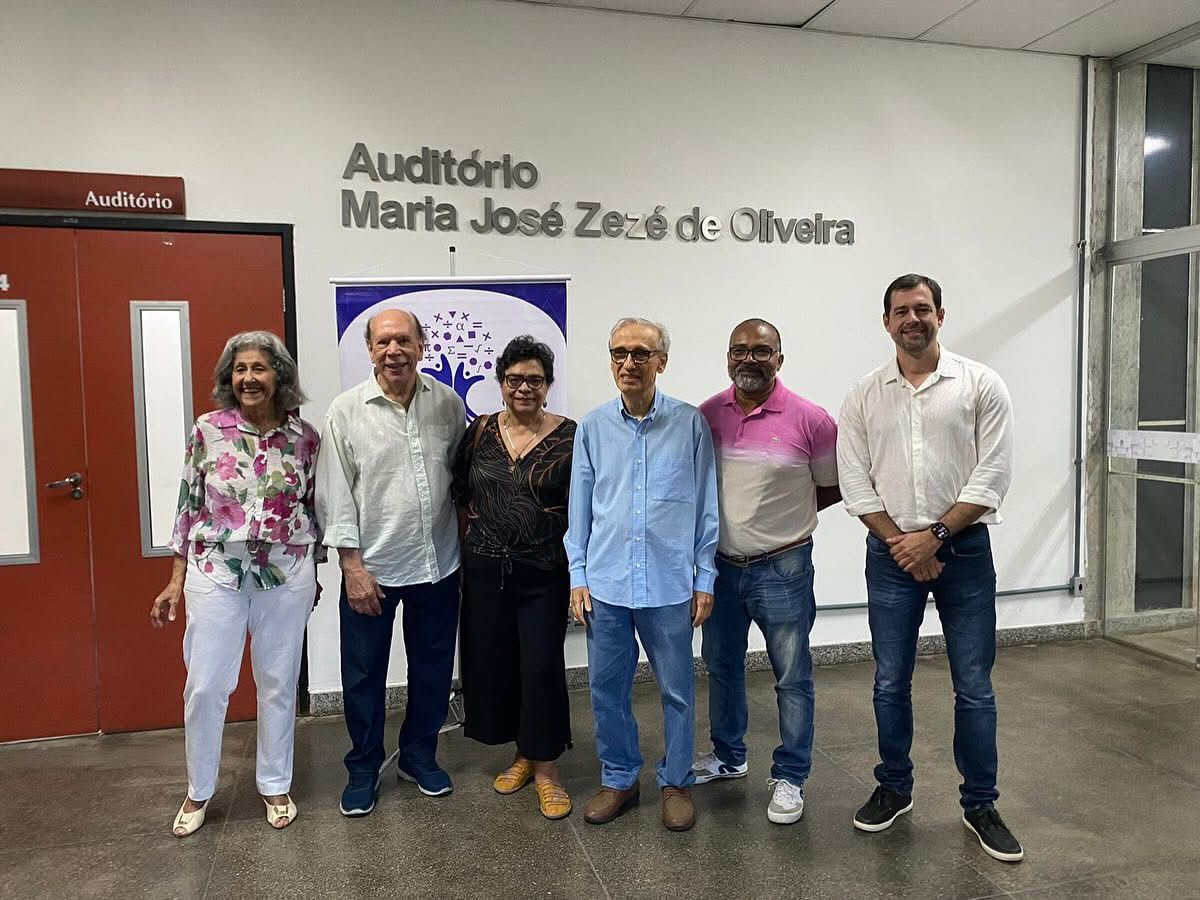
\includegraphics[width=8cm]{Encontro.jpeg}
\end{center}
\caption{O atual diretor e outros ex-diretores do IME: 
 Célia Maria Pitangueira Gomes, Adelmo Ribeiro de Jesus, 
 Ilka Rebouças Freire, José Fernandes Silva Andrade, 
 Evandro Carlos Ferreira dos Santos e Kleyber Mota da Cunha.
}
\end{figure}

Na parte acadêmica, fiz concurso para Professor Titular em
agosto de 1999, do qual constaram Prova de Títulos, Defesa
de Memorial e Conferência na área do concurso. No começo do
ano seguinte, assumi como Professor Titular. Durante todo o
período em que fui diretor, apesar de não ter obrigação,
sempre lecionei uma disciplina, todas no primeiro horário da
manhã, para que as tarefas da direção não prejudicassem as
minhas aulas. É importante mencionar que dar aula sempre foi
o que mais gostei de fazer durante todo o meu tempo de
professor. Orientei mais dois alunos em suas Dissertações de
Mestrado, tendo um deles concluído o seu trabalho em 1998, e
o outro em 1999. A orientação na iniciação científica
continuou initerruptamente, com pelo menos dois alunos em
cada ano.

Em 1998, participei pela primeira vez de uma atividade de
extensão, ministrando aulas para professores da UNEB, na
cidade de Senhor do Bonfim. No ano seguinte, no projeto
Pró-Ciências no Instituto de Matemática, ministrei um curso
sobre Análise Combinatória. Ele foi repetido em 2000 e 2001.
Nessa época, já tinha sido criado o LEMA, com modelos
concretos, principalmente na área de Geometria e um pouco na
de Álgebra Elementar. Como eu ministrava as aulas de Análise
Combinatória sempre fazendo desenhos ou modelos no quadro
para que essa visualização tornasse mais fácil a compreensão
e solução dos problemas pelos alunos, propus à Profa.
Elinalva Vasconcelos, Coordenadora do LEMA
na época, %revH
a construção de
modelos concretos que ajudassem os alunos na solução dos
problemas de Análise Combinatória. Dessa maneira, o LEMA
ganhou os primeiros modelos nesta área. Eles foram
construídos pela artista Fabiana Laranjeiras. Daí até a
minha aposentadoria, participei de vários projetos de
extensão.

Na época em que estava na direção do Instituto, resolvi
escrever um artigo para ser submetido para publicação na
revista Matemática Universitária da SBM, contendo alguns
contraexemplos simples em espaços vetoriais de dimensão
infinita, de resultados válidos nos espaços vetoriais de
dimensão finita. Eu já tinha elaborado esses contraexemplos
em 1990, quando ensinei pela primeira vez a disciplina
Álgebra Linear II da graduação, mas nunca tinha escrito de
uma forma que pudesse ser publicado. O artigo foi aceito e
publicado no volume 37 do ano de 2004.

Em setembro de 2000, como membro do Conselho Universitário
da UFBA, fui indicado para ser um dos três representantes
deste Conselho no Conselho de Curadores, tendo sido um dos
seus membros até o final do meu mandato de Diretor, quando
também se encerrou minha participação no Conselho
Universitário e, consequentemente, também no Conselho de
Curadores. Participei então dos três Conselhos da
Universidade que havia no meu tempo de professor: Conselho
de Coordenação, depois CONSEPE, Conselho Universitário e
Conselho de Curadores.





\begin{center}\emph{2003--2011}\end{center}



Foi durante o tempo em que fui Diretor do Instituto que
começaram regularmente na UFBA os concursos para a classe de
Professor Adjunto, que exige para entrada o grau de Doutor.
Com isso, o Corpo Docente do Curso de Mestrado foi
aumentando. Consequentemente, mudaram um pouco as minhas
atividades no Departamento de Matemática. Continuei
lecionando duas disciplinas a cada semestre, sendo a última
no Curso de Mestrado em 2007. A partir daí, só lecionei
disciplinas na graduação, sempre disciplinas específicas do
Curso de Matemática. É interessante observar que todas as
disciplinas que lecionei nesse período foram da área de
Álgebra ou Variáveis Complexas ou Análise Combinatória,
todas relacionadas com o meu doutorado: a área de Álgebra
foi a área do doutorado, Variáveis Complexas a segunda área
do exame de qualificação, e utilizei fortemente Análise
Combinatória no último capítulo da tese. Usei também
Combinatória na demonstração de alguns teoremas em trabalhos
que publiquei, entre eles um artigo de pesquisa com Aron
Simis. Não posso deixar de mencionar aqui que, depois que
entrei na universidade como aluno em 1971, o único curso que
fiz sobre o assunto de Análise Combinatória foi na minha
graduação: a disciplina Estatística III-C, lecionada pela
Profa. Margot Piva, excelente professora do Departamento de
Estatística.

As orientações de iniciação científica foram até 2005.
Recebi nesse ano uma homenagem da UFBA pela minha
participação destacada nos Seminários Estudantis de Pesquisa
da UFBA que estava completando 25 anos. Também fui Professor
Homenageado ou Patrono em cinco solenidades de formatura do
Curso de Graduação em Matemática.

No final de 2004, fui indicado para mais um mandato no
CONSEPE, sendo reconduzido na representação para um segundo
período, participando desse Conselho de janeiro de 2005 a
dezembro de 2008. 

\begin{figure}[htb!]
\begin{center}
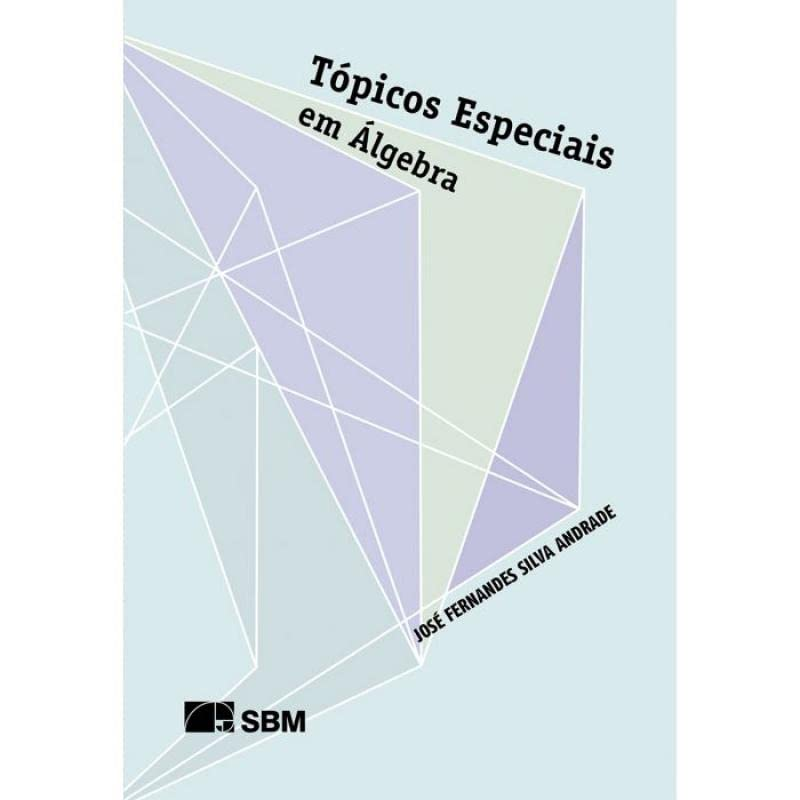
\includegraphics[width=9.5cm]{livro.png}
\end{center}
\caption{``O livro de José Andrade facilita 
o ensino e a aprendizagem em disciplinas 
de álgebra. Os resultados expostos são baseados 
em sua experiência na graduação, em atividades 
de iniciação científica e no mestrado. Portanto, 
os alunos podem aprofundar seus estudos em 
tópicos como anéis de ideais principais, 
anéis de inteiros quadráticos, além de domínios euclidianos, 
unicidade no algoritmo da divisão, soma de quatro 
quadrados, triângulos retângulos com 
lados inteiros e o último teorema de Fermat.'' (resumo
extraído do \emph{site} da SBM.)}   
\end{figure}

Apresentei um projeto que foi aprovado pelo Departamento
para escrever uma série de artigos sobre assuntos que
complementam tópicos das diversas disciplinas do Curso de
Graduação em Matemática na Área de Álgebra. Os dois
primeiros, Triângulos Retângulos com Lados Inteiros:
Procurando as Hipotenusas e Anéis Quadráticos Euclidianos
foram publicados na revista Matemática Universitária nos
volumes 41 e 48/49 dos anos de 2006 e 2010, respectivamente.
Depois, resolvi escrever um livro sobre esse tema no qual
inclui todo o material publicado nos três artigos que
escrevi para a Matemática Universitária. Quando me aposentei
em 2011, o livro não estava ainda todo escrito, mas continuei
com o projeto. O livro Tópicos Especiais em Álgebra ficou
pronto e foi publicado pela SBM, na Coleção Iniciação
Científica, no começo de 2014. São doze capítulos com tópicos
independentes. Dediquei-o à minha esposa Profa. Ednalva
Andrade, colega, amiga, parceira, que contribuiu muito para
a minha carreira e a quem presto mais uma homenagem nestas
notas. Fiz seu lançamento no auditório do Instituto de
Matemática. O ponto mais importante foi a apresentação que
fiz no auditório: convidei professores, ex-professores,
alunos, ex-alunos, amigos e familiares. Disse a todos que
falaria para os meus amigos não matemáticos. Fiquei muito
feliz com o evento. De todos os meus trabalhos publicados,
esse foi um dos que mais gostei de ter escrito, só perdendo
para a minha tese de doutorado. 

\vfill
\begin{wrapfigure}{L}{1.7cm}
\vspace{-10pt}
  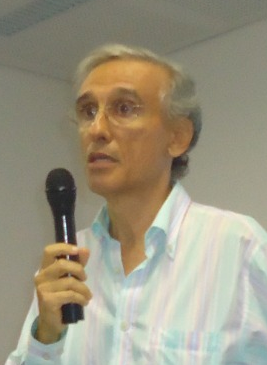
\includegraphics[width=2cm]{fotobio.png}
\end{wrapfigure}\noindent
José Fernandes nasceu em  Salvador, obteve o doutorado
em Álgebra no IMPA e é professor aposentado da UFBA, 
onde também se graduou. 
Além da matemática, uma das coisas que gosta de fazer é
passear e tomar sorvete na Ribeira, onde morou até um 
ano antes de completar a graduação.

\end{document}
